% =========================================================================
% Beyond Top-K: A Typed Operator Suite for Answer-Geometry Mismatches in KGQA
%
% Draft v12.1 (2026-06-01) -- v12 reframed around answer-geometry mismatch
% and operator-driven gain (advice-driven revision over v11); v12.1 merges
% Limitations / Future Work / Appendix robustness from v5_revised.
% Full v10 manuscript: strategy_routed_graphrag_full.tex
%
% Compile with XeLaTeX (Chinese characters in text/tables).
% =========================================================================
\documentclass[10pt,a4paper,twocolumn]{article}

\usepackage[margin=1.9cm]{geometry}
\usepackage[T1]{fontenc}
\usepackage{microtype}
\usepackage{graphicx}
\usepackage{booktabs}
\usepackage{amsmath,amssymb}
\usepackage{array}
\usepackage{makecell}
\usepackage{multirow}
\usepackage{xcolor}
\usepackage{enumitem}
\usepackage{natbib}
\usepackage[hidelinks]{hyperref}
\usepackage{pifont}
\newcommand{\cmark}{\ding{51}}
\newcommand{\xmark}{\ding{55}}

% Chinese support
\usepackage{xeCJK}
\IfFontExistsTF{SimSun}{%
  \setCJKmainfont{SimSun}%
  \setCJKsansfont{SimSun}%
  \setCJKmonofont{SimSun}%
}{%
  \IfFontExistsTF{Noto Serif CJK SC}{%
    \setCJKmainfont{Noto Serif CJK SC}%
    \setCJKsansfont{Noto Serif CJK SC}%
    \setCJKmonofont{Noto Serif CJK SC}%
  }{}%
}

% Better URL / path handling for long technical strings
\usepackage{xurl}        % allows breaking URLs at almost any character
\sloppy                  % allows looser line breaks for overfull boxes

\setlength{\parskip}{0.4em}
\setlength{\parindent}{0pt}
\renewcommand{\arraystretch}{1.05}

\newcommand{\qtype}[1]{\texttt{\small #1}}
\newcommand{\op}[1]{\textsc{\small #1}}

\title{Beyond Top-K: \\
A Typed Operator Suite for Answer-Geometry Mismatches in Knowledge Graph QA}

\author{TBD \\ \small{Draft v12.1, 2026-06-01}}
\date{}

\begin{document}
\maketitle

% =========================================================================
\begin{abstract}
GraphRAG systems converge on increasingly sophisticated top-$K$ retrieval algorithms --- community summarization, Personalized PageRank, LLM path templates, beam search --- but top-$K$ embeds an implicit assumption about \emph{answer geometry}: that the answer is a small set rankable by surface relevance. This assumption systematically fails on three computable patterns common in industrial KGs --- unbounded enumeration, multi-constraint intersection, and complement / non-membership --- for \emph{information-theoretic} reasons, not LLM-capacity reasons. We identify this \textbf{answer-geometry mismatch} as analogous to the OLTP/OLAP split in databases: a B-tree index is excellent for point queries and structurally wrong for aggregate queries, regardless of how it is tuned. We propose \textbf{Strategy-Routed GraphRAG}, a typed suite of six retrieval operators (\op{lookup}, \op{exhaustive}, \op{complement}, \op{path-plan}, \op{constrained-join}, \op{dual-subgraph}), each \emph{derived} as the primitive satisfying its target class's information requirement. The dispatcher is a lightweight LLM lookup; an \textbf{oracle ablation localizes the entire gain to the operators} (88.2\% oracle vs 88.6\% LLM dispatch, $\Delta\!=\!-0.4$ pp) --- \textbf{this is a paper about the operators, not the classifier}. On \textbf{RadarKG-QA-499}, a new bilingual benchmark we release explicitly designed to expose answer-geometry mismatch (3.4$\times$ the median Count cardinality of public benchmarks), the suite reaches \textbf{88.6\%} vs Baseline 52.7\% and a zero-shot path planner 60.3\% ($+35.9$ / $+28.3$ pp, paired bootstrap CIs strict-positive, robust to $K{=}8{\to}20$). Cross-domain on KQA Pro the typology and dispatcher transfer for free (67.4\% routing match without retraining; \op{dual-subgraph} $+11$ pp on SelectBetween); the absolute gain scales with how much of a benchmark exhibits answer-geometry mismatch --- public benchmarks systematically under-sample this regime, which we document as a community gap. At \$0.00041/Q (\$0.00084 per accuracy-point), the suite is deployable for industrial KGQA.
\end{abstract}

% =========================================================================
\section{Introduction}
\label{sec:intro}

\paragraph{Phenomenon.}
Industrial deployments of GraphRAG \citep{edge2024graphrag,gutierrez2024hipporag,luo2024rog,sun2024tog,ma2025tog2} face a stubborn distribution of queries that uniformly applied top-$K$ retrieval cannot answer. Consider three natural questions on a radar KG:

\begin{table*}[h]
\centering
\small
\begin{tabular}{p{0.43\linewidth}|p{0.49\linewidth}}
\toprule
\textbf{Question shape} & \textbf{Why top-$K$ fails} \\
\midrule
\emph{``How many radars does the US operate?''} & Answer set has $>$400 elements; no $K$ bounded by retrieval budget enumerates it. \\
\emph{``Radars by US firms AND in S band.''} & Top-$K$ cannot express \emph{intersection} across constraints. \\
\emph{``Is AN/TPY-2 exported to Japan?''} & KG announces presence, not absence; top-$K$ misses non-local negation. \\
\bottomrule
\end{tabular}
\end{table*}

These are not LLM failures: regardless of model capacity, top-$K$ cannot enumerate 400 answers when $K\!=\!8$, cannot express AND across two independent ranking signals, and cannot announce absence in a KG that stores only presence. They are \emph{information-theoretic} failures --- the retrieved set lacks the bits any downstream reasoner would need. In RadarKG-QA-499 (§\ref{sec:benchmark}), ${\sim}30\%$ of natural questions fall in these classes; baseline top-$K$ scores 4--12\% on them regardless of LLM choice or $K \in \{8, 20\}$ (§\ref{sec:rq1}, Table~\ref{tab:k20}).

\paragraph{Diagnosis: Answer-Geometry Mismatch.}
Top-$K$ embeds an implicit assumption about \emph{answer geometry} --- that the answer is a small set rankable by surface relevance to the query. This assumption holds for factoid queries (the canonical evaluation regime of WebQSP and NaturalQuestions). It fails on three computable patterns common in industrial KGs:
\begin{itemize}[topsep=0pt,itemsep=0pt,leftmargin=*]
  \item \textbf{Unbounded enumeration} (counting, list-all): information requirement is the \emph{complete set}; top-$K$ is bounded by $K$.
  \item \textbf{Multi-constraint intersection} (AND across independent ranking signals): information requirement is \emph{set intersection}; top-$K$'s ranking conflates the constraints.
  \item \textbf{Complement / non-membership} (confirming absence): information requirement is \emph{global negation}; the KG stores only positive triples, so absence is not present in any local window.
\end{itemize}
We call this \textbf{answer-geometry mismatch} (AGM): the query's information requirement is structurally incompatible with what top-$K$'s geometry can deliver. Whether 30\% or 5\% of a benchmark exhibits AGM is a property of the \emph{benchmark distribution}, not of top-$K$ itself --- public benchmarks systematically under-sample this regime (§\ref{sec:bench-design}, Table~\ref{tab:bench-distribution}); industrial KGs systematically over-sample it.

\paragraph{Insight: Match Information Requirement to Operator.}
The pattern is familiar from database theory. A B-tree index is excellent for point queries (\texttt{SELECT WHERE id\!=\!5}) and a structurally inappropriate execution plan for aggregate queries (\texttt{COUNT(*) GROUP BY country}) --- not because B-trees are bad, but because the query's information requirement requires a different access pattern. Databases respond not by improving the B-tree but by adding \emph{typed execution plans} (hash join, full scan, sort-merge) and a query optimizer that picks the right one. \textbf{Top-$K$ is the B-tree of GraphRAG}: optimal for factoid retrieval, structurally mismatched for analytical KGQA. The fix is not a better ranker --- it is the \emph{right operator for each query's information requirement}. We enumerate the information-requirement classes that top-$K$ cannot satisfy and derive a typed suite of six operators (§\ref{sec:method}). A lightweight LLM dispatcher maps each question to its operator class.

\paragraph{System (and the Oracle Surprise).}
We instantiate the framework as \textbf{Strategy-Routed GraphRAG}: an LLM dispatcher + six typed operators + an LLM answerer reading the operator's evidence. The dispatcher reaches 93\% type-classification accuracy zero-shot --- but its accuracy is not load-bearing. \textbf{An oracle ablation replacing the LLM dispatcher with gold question-type routing reaches 88.2\% end-to-end vs the LLM dispatcher's 88.6\% ($\Delta\!=\!-0.4$ pp; §\ref{sec:rq3})}: the entire $+35.9$ pp gain over baseline is operator-driven, not dispatcher-driven. \textbf{This is a paper about the operators, not the classifier.} The dispatcher is an $O(1)$ table lookup that an LLM happens to solve well; the analytical contribution is the operator suite that satisfies the information requirements top-$K$ cannot meet.

\paragraph{Contributions.}
\textbf{(1)} \textbf{Answer-geometry mismatch diagnosis}: a precise account, grounded in information-theoretic minima, of when and why top-$K$ retrieval systematically fails on KGQA, framed via the OLTP/OLAP analogy from database theory --- transferable beyond the radar domain.
\textbf{(2)} \textbf{A typed suite of six retrieval operators}, each derived as the primitive satisfying its target class's information requirement. The dispatcher is shown empirically to contribute ${\approx}0$ pp; the operators carry the gain.
\textbf{(3)} \textbf{RadarKG-QA-499}, the first KGQA benchmark explicitly designed to expose AGM (3.4$\times$ higher median Count cardinality than public benchmarks), with a 26-Q OOD bilingual stress subset.
\textbf{(4)} \textbf{Empirical}: $+35.9$ pp over baseline, $+28.3$ pp over single-policy path planning on all 499 questions, with paired bootstrap CIs and ablations (retrieval-budget, per-operator, suite-size, oracle-dispatcher, cross-domain) that localize the gain to operator design.
\textbf{(5)} \textbf{Methodological finding}: in-distribution evaluation of bilingual / alias-handling components yields false-negative ablations (§\ref{sec:rq3}); a 0 pp $\to$ $+11.5$ pp gap appears on an OOD stress set, calling for dedicated alias-OOD evaluation in multilingual KGQA.

% =========================================================================
\section{Method}
\label{sec:method}

\subsection{Pipeline}
A question is processed by three LLM stages --- \textbf{dispatcher} (selects an operator), \textbf{parser} (extracts entities and relation chain), \textbf{answerer} (renders evidence into a natural-language answer) --- and one KG-only \textbf{executor} (Fig.~\ref{fig:pipeline}). The KG (RadarKG-v2: 16{,}513 triples, 98 relations + attributes, 4{,}827 entities) is queried only in the executor, never via LLM.

\begin{figure}[h]
\centering
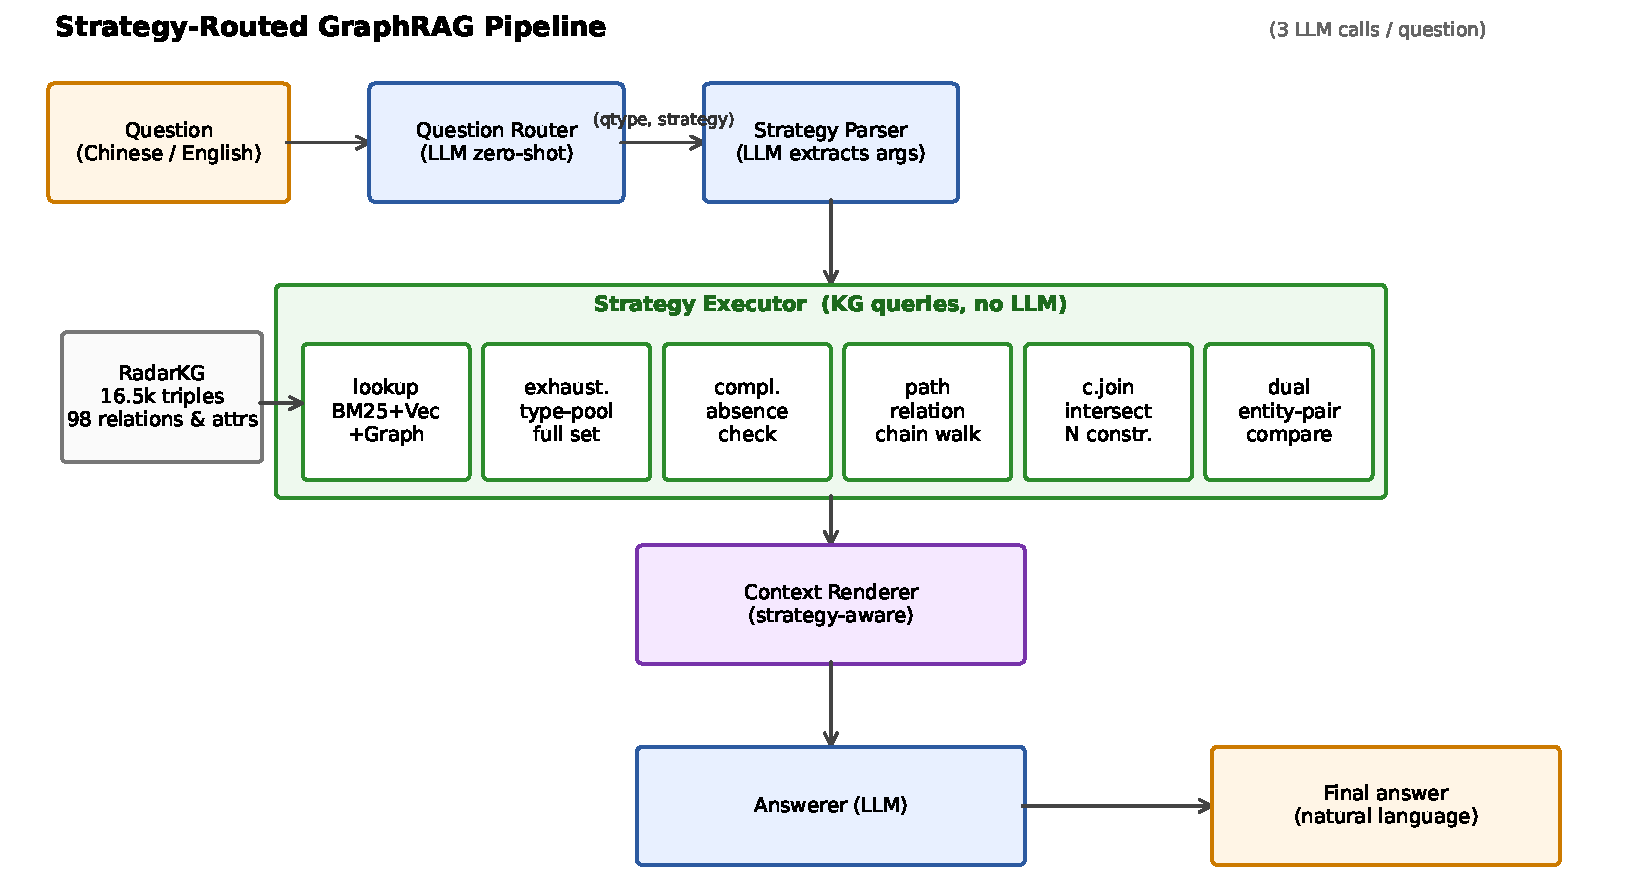
\includegraphics[width=0.95\linewidth]{figures/fig1_pipeline.pdf}
\caption{Strategy-Routed GraphRAG pipeline.}
\label{fig:pipeline}
\end{figure}

\subsection{Question Typology}
We define 11 question types grounded in the \emph{retrieval pattern} each requires (not surface form). Each type deterministically maps to one operator.

\begin{table*}[h]
\centering
\small
\caption{11-way typology $\to$ 6-operator mapping.}
\label{tab:typology}
\begin{tabular}{p{0.35\linewidth} p{0.25\linewidth} l}
\toprule
\textbf{Type} & \textbf{Signal} & \textbf{Operator} \\
\midrule
\qtype{single\_hop}                                                 & entity + attr     & \op{lookup} \\
\qtype{relation\_inverse,} \qtype{agg\_count,} \qtype{agg\_enum}    & unbounded enum    & \op{exhaustive} \\
\qtype{two\_hop\_bridge,} \qtype{three\_hop\_chain}                 & composition $k\!\geq\!2$ & \op{path-plan} \\
\qtype{attr\_filter}                                                & AND of constraints & \op{constrained-join} \\
\qtype{negation,} \qtype{unanswerable}                              & absence            & \op{complement} \\
\qtype{set\_compare}                                                & two entities       & \op{dual-subgraph} \\
\qtype{distractor}                                                  & disambiguation     & \op{lookup} \\
\bottomrule
\end{tabular}
\end{table*}

\subsection{Deriving the Operator Suite from Information Requirements}
\label{sec:derivation}

We do not choose operators by inspection of common failure modes. We enumerate the \emph{information-requirement classes} that top-$K$ cannot satisfy and derive an operator for each, then add \op{lookup} for the class top-$K$ \emph{does} satisfy. Table~\ref{tab:reqs} makes the derivation explicit; Table~\ref{tab:operators} gives implementation mechanisms.

\begin{table*}[t]
\centering
\small
\caption{Information-requirement derivation of the operator suite. Each row determines its operator by the minimal access pattern satisfying the requirement; top-$K$ fails for a different reason in each row.}
\label{tab:reqs}
\setlength{\tabcolsep}{4pt}
\begin{tabular}{p{0.18\linewidth} p{0.27\linewidth} p{0.28\linewidth} p{0.20\linewidth}}
\toprule
\textbf{Pattern} & \textbf{Information requirement (minimal)} & \textbf{Why top-$K$ fails} & \textbf{Derived operator} \\
\midrule
Identity / factoid     & one best-matching triple                                 & (none --- top-$K$ satisfies this)                                & \op{lookup} = BM25 $\oplus$ vec $\oplus$ RRF \\
Unbounded enumeration  & \emph{complete} head/tail set for a relation             & $K$ is an upper bound; answer set is not                         & \op{exhaustive} = $\{h \mid (h,r,t)\!\in\!\text{KG}\}$ \\
Multi-constraint AND   & set intersection of $N$ relations' head sets             & ranking cannot express AND; conflates signals                    & \op{constrained-join} = $\bigcap_i \text{heads}(r_i,t_i)$ \\
Complement / absence   & complete \emph{known} set, then explicit gap             & KG stores only positive facts; absence is non-local              & \op{complement} = enumerate then verify \\
Composition $(k\!\geq\!2)$ & path through $k$ relations preserving hop structure & top-$K$ is flat; loses hop boundaries                            & \op{path-plan} = $\text{tails}_{r_1}\!\circ\!\dots\!\circ\!\text{tails}_{r_k}$ \\
Binary comparison      & \emph{both} sides' subgraphs explicit and aligned        & top-$K$ may starve one side; cannot align                        & \op{dual-subgraph} = parallel $\text{tails}(A,B)$ + set ops \\
\bottomrule
\end{tabular}
\end{table*}

Each operator is the \emph{minimal} access pattern that meets its row's information requirement: dropping ``exhaustive'' from \op{exhaustive} reintroduces the $K$-bounded failure; dropping the intersection from \op{constrained-join} recovers the conflated-ranking failure; and so on. The derivation justifies both the \emph{number} (six requirement classes, six operators) and the \emph{content} of the suite --- neither is empirical curve-fitting. The empirical question is whether \emph{additional} classes exist in practice; §\ref{sec:rq2}'s suite-size ablation answers this (the three load-bearing operators have additive contributions on disjoint question slices; a 4-operator subset matches the full 6-op accuracy on this benchmark).

\paragraph{Scope of the derivation claim.}
The framework above is \emph{grounded} in matching information requirements to access patterns; we do not claim \emph{formal completeness}. The six requirement classes were identified by inspection of common KGQA failure modes on our radar benchmark and are not a closed taxonomy: further patterns --- aggregation arithmetic (\texttt{SUM}, \texttt{AVG} over numeric properties), transitive closure, temporal-range constraints, fuzzy matching --- would motivate additional operators (Discussion §\ref{sec:discussion} sketches the extension path). The derivation gives the suite a principled \emph{origin} but not a proof of \emph{minimality} or \emph{coverage} in any algebraic sense.

\begin{table*}[t]
\centering
\small
\caption{Six-operator suite --- implementation mechanisms.}
\label{tab:operators}
\begin{tabular}{l p{0.78\linewidth}}
\toprule
\textbf{Operator} & \textbf{Mechanism} \\
\midrule
\op{lookup}            & BM25 + bi-encoder + RRF + 2-hop graph expansion; (head, relation) bypass via KG-direct lookup for parser-extracted args. \\
\op{exhaustive}        & $\{h \mid (h, r, t) \in \text{KG}\}$, no $K$ cutoff. Equivalence-class fallback (below) on empty result. \\
\op{complement}        & Enumerate $\{t \mid (h, r, t) \in \text{KG}\}$; flag empty / non-membership so the LLM emits explicit ``否'' rather than hallucinate. \\
\op{path-plan}         & Relation-chain BFS with inverse traversal $r^{-1}$, returning terminal entities and full edge trace. \\
\op{constrained-join}  & Head-set intersection across $N$ constraints with \textbf{equivalence-class fallback}: unions semantically equivalent relations (e.g., \texttt{countryOfOrigin}\,$\cup$\,\texttt{operatedBy}) on empty intersection --- addresses disjoint-subgraph noise from multi-source extraction. \\
\op{dual-subgraph}     & Parallel \textit{tails\_of} on $(A,B)$ over a shared relation, rendered side-by-side with $A\!\cap\!B$, $A{\setminus}B$, $B{\setminus}A$ pre-computed. \\
\bottomrule
\end{tabular}
\end{table*}

The \op{lookup} operator additionally serves as a safe fallback for dispatcher errors: misrouted questions degrade to standard hybrid retrieval rather than to a wrong operator's empty result.

\subsection{Dispatcher and Bilingual Alias Layer}
A zero-shot DeepSeek-Chat router with typology definitions + 5 examples maps question $\to$ type $\to$ operator. Routing accuracy 93.0\%. A cross-cutting \textbf{bilingual alias layer} (5-stage cascade: direct match $\to$ 614-form alias index $\to$ frequency-band normalization $\to$ suffix stripping $\to$ equivalence-class union) handles industrial Chinese KGs with mixed-language values.

% =========================================================================
\section{Benchmark: RadarKG-QA-499}
\label{sec:benchmark}

\subsection{Knowledge Graph}
RadarKG-v2 has 4{,}827 entities and 12{,}219 inter-entity edges + ${\sim}80$ typed properties, built from a 472-page airborne-radar handbook (full OCR), Wikidata SPARQL pulls, and Wikipedia summaries. Country-of-origin and developer coverage: 93.4\% / 87.0\%. Schema is English; value vocabulary is mixed Chinese-English.

\subsection{Question Generation}
We auto-generate 499 questions stratified across the 11 types, each with machine-verifiable gold (Table~\ref{tab:qa-dist}). An additional \textbf{26-Q OOD bilingual stress subset} substitutes English/abbreviation aliases into Chinese templates to isolate the alias layer.

\begin{table*}[h]
\centering
\small
\caption{RadarKG-QA-499 distribution.}
\label{tab:qa-dist}
\begin{tabular}{l r l r}
\toprule
\textbf{Type} & \textbf{n} & \textbf{Type} & \textbf{n} \\
\midrule
\qtype{single\_hop}        & 80 & \qtype{attr\_filter}      & 50 \\
\qtype{two\_hop\_bridge}   & 80 & \qtype{negation}          & 40 \\
\qtype{relation\_inverse}  & 50 & \qtype{set\_compare}      & 40 \\
\qtype{agg\_count}         & 50 & \qtype{three\_hop\_chain} & 30 \\
\qtype{agg\_enum}          & 50 & \qtype{unanswerable}      & 20 \\
                           &    & \qtype{distractor}        & 9  \\
\midrule
\multicolumn{3}{l}{\textbf{Total}} & \textbf{499} \\
\bottomrule
\end{tabular}
\end{table*}

\subsection{Why a New Benchmark}
\label{sec:bench-design}
We claim RadarKG-QA-499 is a \emph{primary} contribution because no public KGQA benchmark currently stratifies for high-cardinality answer sets --- the cleanest signal of retrieval-budget structural failure.

\begin{table*}[h]
\centering
\small
\caption{Cross-benchmark Count answer cardinality. RadarKG-QA-499 has 3.4$\times$ the median and 3$\times$ the high-cardinality fraction of the next-closest public benchmark.}
\label{tab:bench-distribution}
\begin{tabular}{l r r r r}
\toprule
\textbf{Benchmark} & \textbf{n} & \textbf{Med.} & \textbf{Mean} & \textbf{\% $\!\geq\! 30$} \\
\midrule
\textbf{RadarKG-QA-499} & 50 & \textbf{14} & \textbf{25.3} & \textbf{18\%} \\
KQA Pro val            & 1318 & 2 & 11.7 & 6\% \\
KQA Pro pure-enum      & 557 & 1 & 3.7  & 2\% \\
Mintaka dev            & 200 & 4 & 7.1  & 3\% \\
WebQSP                 & \multicolumn{4}{c}{88\% single-hop (no count emphasis)} \\
LC-QuAD 2.0            & \multicolumn{4}{c}{requires live SPARQL execution} \\
\bottomrule
\end{tabular}
\end{table*}

The same gap holds at \qtype{attr\_filter} (multi-constraint) and \qtype{three\_hop\_chain}. We release RadarKG-QA-499 to fill this gap.

% =========================================================================
\section{Experiments}
\label{sec:experiments}

\paragraph{Setup.} All systems use DeepSeek-Chat \citep{deepseekv3_2024}. Three systems: \textbf{Baseline} = BM25 \citep{robertson2009bm25} + bi-encoder \citep{xiao2024bge} + RRF \citep{cormack2009rrf} + 2-hop expansion, top-$K\!=\!8$; \textbf{Zero-shot Path Planner (RoG-inspired)} = our zero-shot reproduction of single-policy LLM-emitted path planning; \textbf{Strategy} = our pipeline. All evaluated on all 499 questions; paired bootstrap CIs (1000 resamples).

\paragraph{RoG comparison caveat.}
We abbreviate the second system as \textbf{RoG} in tables. The main-table RoG column is a \emph{zero-shot} path planner (DeepSeek) --- not a faithful reproduction of \citet{luo2024rog}, which fine-tunes a planner. We deliberately separate the \emph{single-policy uniform-application} assumption (what we critique) from supervised path emission (orthogonal). \textbf{To rule out a weak-baseline artifact, §\ref{sec:rq6} reports faithful fine-tuned planners on two bases} (LoRA on KG-mined paths), including the original RoG base LLaMA-2-7B-Chat: fine-tuning improves each ${\sim}{+}30$ pp over its zero-shot baseline, yet Strategy still leads the best variant by $+27$ to $+33$ pp on the same structural grounds --- robust to base-model choice.

\subsection{RQ1: Does Strategy beat single-policy retrieval?}
\label{sec:rq1}

\begin{table*}[t]
\centering
\small
\caption{Main results on RadarKG-QA-499 (n$\,=\,$499, accuracy \% with 95\% paired bootstrap CI). Strategy wins on 9/11 categories with strict-positive CIs.}
\label{tab:main}
\setlength{\tabcolsep}{3.5pt}
\begin{tabular}{l r l l l l l}
\toprule
\textbf{Type} & \textbf{n} & \textbf{Baseline} & \textbf{RoG} & \textbf{Strategy} & \textbf{$\Delta$ S$-$B} & \textbf{$\Delta$ S$-$RoG} \\
\midrule
\qtype{agg\_count}        & 50 & 4.0 [0, 10] & 38.0 [26, 50] & \textbf{62.0 [48, 74]} & $+$58 [$+$44, $+$72] & $+$24 [$+$12, $+$36] \\
\qtype{agg\_enum}         & 50 & 46.0 [32, 58] & 92.0 [84, 98] & \textbf{96.0 [90, 100]} & $+$50 [$+$36, $+$64] & $+$4 [$+$0, $+$10] \\
\qtype{attr\_filter}      & 50 & 12.0 [4, 22]  & 0.0           & \textbf{92.0 [84, 98]} & $+$80 [$+$66, $+$92] & $+$92 [$+$84, $+$98] \\
\qtype{relation\_inverse} & 50 & 40.0 [26, 54] & 74.0 [62, 86] & \textbf{86.0 [76, 94]} & $+$46 [$+$32, $+$60] & $+$12 [$+$4, $+$22] \\
\qtype{three\_hop\_chain} & 30 & 23.3 [10, 40] & 50.0 [33, 70] & \textbf{93.3 [83, 100]} & $+$70 [$+$53, $+$87] & $+$43 [$+$23, $+$63] \\
\qtype{two\_hop\_bridge}  & 80 & 40.0 [29, 51] & \textbf{95.0 [90, 99]} & 88.8 [81, 95] & $+$49 [$+$38, $+$60] & $-$6 [$-$14, $+$0] \\
\qtype{single\_hop}       & 80 & 83.8 [75, 91] & 11.2 [5, 19]  & \textbf{86.2 [79, 94]} & $+$2.5 [$+$0, $+$6] & $+$75 [$+$65, $+$85] \\
\qtype{set\_compare}      & 40 & 97.5 [93, 100] & 85.0 [73, 95] & 97.5 [93, 100] & 0 & $+$13 [$+$3, $+$23] \\
\qtype{negation}          & 40 & 100.0          & 97.5 [93, 100] & 100.0 & 0 & $+$3 [$+$0, $+$8] \\
\qtype{unanswerable}      & 20 & 90.0 [75, 100] & \textbf{100.0} & 90.0 [75, 100] & 0 & $-$10 [$-$25, $+$0] \\
\qtype{distractor}        & 9  & 100.0          & 66.7 [33, 100] & 100.0 & 0 & $+$33 [$+$0, $+$67] \\
\midrule
\textbf{OVERALL} & \textbf{499} & \textbf{52.7 [48, 57]} & \textbf{60.3 [56, 65]} & \textbf{88.6 [86, 91]} & \textbf{$+$35.9 [$+$32, $+$40]} & \textbf{$+$28.3 [$+$24, $+$33]} \\
\bottomrule
\end{tabular}
\end{table*}

The two ``losses'' (\qtype{two\_hop\_bridge} $-$6 pp, \qtype{unanswerable} $-$10 pp) have CIs touching zero --- ties, not losses. RoG underperforms baseline on \qtype{single\_hop} ($-$72.5 pp), \qtype{distractor} ($-$33 pp), \qtype{attr\_filter} ($-$12 pp): uniform path planning is \emph{worse} than no planning when no path is needed.

\paragraph{Retrieval-budget ablation.}
A $K\!=\!8 \to K\!=\!20$ baseline change lifts Baseline only $+2.4$ pp $[+0.0, +4.6]$ (Table~\ref{tab:k20}); Strategy still wins $+33.5$ pp $[+29.5, +37.9]$ over the $K\!=\!20$ baseline. Categories where Strategy wins biggest gain $\leq 6$ pp from $K\!=\!20$: \qtype{agg\_count} 4\%$\to$8\%, \qtype{three\_hop\_chain} 23\%$\to$20\% (actually drops), \qtype{attr\_filter} 12\%$\to$18\%. \textbf{Adding retrieval budget cannot fix questions where the answer set is structurally larger than any $K$.}

\begin{table*}[h]
\centering
\small
\caption{$K\!=\!20$ baseline ablation.}
\label{tab:k20}
\begin{tabular}{l r l}
\toprule
\textbf{System} & \textbf{Overall} & \textbf{$\Delta$ paired CI} \\
\midrule
Baseline $K=8$  & 52.7\% & --- \\
Baseline $K=20$ & 55.1\% & $+2.4$ [$+0.0$, $+4.6$] vs $K=8$ \\
Strategy        & 88.6\% & $\mathbf{+33.5}$ [$+29.5$, $+37.9$] vs $K=20$ \\
\bottomrule
\end{tabular}
\end{table*}

\subsection{RQ2: Which operators carry the gain? (Structural Failure \texorpdfstring{$\to$}{->} Operator)}
\label{sec:rq2}

We perform per-operator ablation (100-Q subset, force fallback to \op{lookup}; full per-type breakdown in the extended version) and \textbf{explicitly map each operator's contribution to the AGM class it addresses}. The §\ref{sec:derivation} derivation predicts a 1:1 correspondence between an operator and the structural failure mode it fixes; Table~\ref{tab:per-op} verifies it.

\begin{table*}[t]
\centering
\small
\caption{Per-operator ablation, with each operator's $\Delta$ contribution mapped to the AGM class it addresses (1:1 correspondence with the §\ref{sec:derivation} derivation).}
\label{tab:per-op}
\begin{tabular}{l r l p{0.42\linewidth}}
\toprule
\textbf{Drop} & \textbf{$\Delta$} & \textbf{AGM class} & \textbf{Most-affected type (and baseline failure mode)} \\
\midrule
$-$\op{exhaustive}        & $\mathbf{-19}$ & unbounded enum (\textsf{card}) & \qtype{agg\_count}, \qtype{agg\_enum}, \qtype{relation\_inverse} $-$60 pp each (top-$K\!\leq\!K$, answer set $> K$) \\
$-$\op{path-plan}         & $\mathbf{-10}$ & composition $k\!\geq\!2$ (\textsf{comp}) & \qtype{three\_hop\_chain} $-$62.5, \qtype{two\_hop\_bridge} $-$41.7 (top-$K$ is flat, loses hop boundaries) \\
$-$\op{constrained-join}  & $\mathbf{-8}$  & intersection AND (\textsf{card$+$comp}) & \qtype{attr\_filter} $-$90 (top-$K$ ranking conflates two independent constraints) \\
$-$\op{complement}        & 0              & non-membership (\textsf{cmpl}) & (\op{lookup} + LLM graceful-degrades on this bench's negation distribution) \\
$-$\op{dual-subgraph}     & 0              & binary comparison (\textsf{comp}) & (\op{lookup} + LLM graceful-degrades on same/different) \\
\bottomrule
\end{tabular}
\end{table*}

\paragraph{Structural failure decomposition.}
Baseline $= 52.7\%$, Strategy $= 88.6\%$, $\Delta=+35.9$ pp. The three load-bearing operators contribute $-19, -10, -8 = -37$ pp on ablation, accounting for the entire structurally recoverable failure budget; the residual is bilingual-layer recovery $+$ dispatcher graceful-degradation, both characterized in §\ref{sec:rq3}. \textbf{Each load-bearing operator fixes the failure mode predicted by its AGM-class derivation} (§\ref{sec:derivation}). The \op{complement} and \op{dual-subgraph} operators register 0 pp because RadarKG-QA-499's negation / comparison distribution is graceful-degradation friendly for \op{lookup} --- the 0 pp signal is benchmark-distribution-dependent, not operator redundancy (§\ref{sec:discussion}).

\textbf{Suite-size ablation} (the extended version): joint drops add linearly (\op{exhaustive}$+$\op{path-plan} $= -29$ pp $= -19{-}10$), confirming the three load-bearing operators target \emph{disjoint} question slices --- they fix structurally different failure modes, not overlapping ones. A 4-operator suite $\{$\op{lookup}, \op{exhaustive}, \op{path-plan}, \op{constrained-join}$\}$ matches the full 6-op accuracy (94.0\%); \op{lookup}-only floors at 57.0\%.

\subsection{RQ3: Operators vs Dispatcher --- where is the gain?}
\label{sec:rq3}

\paragraph{Oracle-dispatcher ablation.}
Replacing the LLM router with gold question-type $\to$ operator routing reaches \textbf{88.2\%} end-to-end --- \textbf{within 0.4 pp of LLM dispatch (88.6\%)}. Dispatcher noise contributes effectively 0 pp; the entire $+35.9$ pp gain is operator-driven. On \qtype{three\_hop\_chain} LLM dispatch \emph{beats} oracle by 13 pp: a flexible router occasionally re-routes around operator weaknesses (e.g., redundant 3-hop chains to \op{exhaustive}), an inherent graceful-degradation property.

\paragraph{Bilingual alias paradox.}
In-distribution (auto-generated questions reusing KG canonical forms) the alias layer registers 0 pp drop; on a 26-Q handcrafted OOD stress test it prevents $+11.5$ pp of loss (paired CI [$+0.0$, $+26.9$]; borderline at $n\!=\!26$). The 0 pp vs $+11.5$ pp gap is itself a methodological finding: \textbf{in-distribution evaluation of alias-handling components yields false-negative ablations.} Authors evaluating bilingual / alias layers should construct dedicated OOD substitution sets.

\subsection{RQ4: Cross-domain transfer}
\label{sec:rq4}
On \textbf{KQA Pro} (Wikidata) the typology and dispatcher transfer without retraining (67.4\% zero-shot routing match); \op{dual-subgraph} yields $+11$ pp on SelectBetween and \op{exhaustive}/\op{constrained-join} recover the same structural gains. The absolute gain tracks how much of a benchmark exhibits answer-geometry mismatch (per-configuration results in the extended version).

\subsection{RQ5: Answer-geometry exposure predicts \texorpdfstring{$\Delta$}{Delta}}
\label{sec:rq5}
Per-type gains scale with \textbf{answer-geometry exposure}: types with high answer cardinality or multi-hop / intersection / complement composition show the largest $\Delta$ (\qtype{agg\_count}, \qtype{relation\_inverse}, \qtype{three\_hop\_chain}, \qtype{attr\_filter} all $+$40--70 pp), whereas atomic single-step types (\qtype{single\_hop}) show $\sim$0 --- consistent with the diagnosis that the gain comes from satisfying information requirements top-$K$ cannot meet, not from better ranking.

\subsection{RQ6: A fine-tuned planner does not close the gap}
\label{sec:rq6}
To rule out a weak-baseline artifact, we LoRA-fine-tune faithful RoG-style planners on two 7B bases --- LLaMA-2-7B-Chat (the original RoG base) and a Qwen-7B control --- on 240 KG-mined (question, relation-path) pairs disjoint from the eval set, replacing only the planner. Fine-tuning lifts each base ${\sim}{+}30$ pp over its zero-shot self (LLaMA-2 26.5$\to$55.9, Qwen 31.5$\to$61.7), letting it re-derive our single-relation operators type-by-type. \textbf{But a single-path planner cannot express set-algebraic operators} (\qtype{attr\_filter} 28/30 vs Strategy 92; intersection needs two joined paths) and overfits its training path-length distribution; the best fine-tuned variant still trails Strategy by $+27$ to $+33$ pp --- robust to base-model choice.

\subsection{Cost and Latency}
Strategy: 4.8\,s/Q, 3 LLM calls, \$0.00041/Q (\$0.00084 per accuracy-point over Baseline; \$0.00064/pp over RoG). 100K questions/month $\approx$ \$41.

% =========================================================================
\section{Discussion}
\label{sec:discussion}

\paragraph{Why keep 0 pp-drop operators?}
\op{Complement} and \op{dual-subgraph} contribute 0 pp on this bench but we retain them for two reasons. \emph{Principled}: each is the minimal operator satisfying a distinct information-requirement class (non-membership and binary comparison; §\ref{sec:derivation}) --- pruning them collapses the derivation. \emph{Pragmatic}: (i) auditable evidence traces for negation and comparison (deployment value); (ii) adversarial-negation and 3-way-comparison stress sets (Future Work) should surface them; (iii) negligible token cost. The 0 pp signal reflects this benchmark's distribution, not the operators' redundancy.

\paragraph{Composability: toward a query algebra.}
Our 11-way typology maps each question to \emph{one} operator, a deliberately simple dispatch policy. The operators themselves, however, are composable, and many natural questions decompose analytically into a composition that satisfies a layered information requirement:

\begin{table*}[h]
\centering
\small
\caption{Analytical operator compositions for natural questions. In the current implementation, the inner composition is realized inside a single operator (e.g.\ \op{constrained-join} returns counts directly); the decomposition shows the suite is closed under natural compositions.}
\label{tab:composability}
\begin{tabular}{p{0.39\linewidth} p{0.55\linewidth}}
\toprule
\textbf{Natural question} & \textbf{Analytical decomposition} \\
\midrule
\emph{``How many S-band radars are developed in China?''} & \op{exhaustive} $\circ$ \op{constrained-join}(\{band$\!=\!$S\},\{country$\!=\!$China\}) \\
\emph{``Among US radars exported to Japan, which use AESA?''} & \op{constrained-join}(\{tech$\!=\!$AESA\}, \op{path-plan}(US, exportedTo, Japan)) \\
\emph{``Does AN/TPY-2 share a manufacturer with AN/SPY-1?''} & \op{dual-subgraph}(AN/TPY-2, AN/SPY-1; developedBy) $\to$ equality \\
\emph{``Radars whose developer's country is not the US.''} & \op{complement}$_{\text{US}}$(\op{path-plan}(?, developedBy, $m$); $m$, affiliatedTo, ?) \\
\bottomrule
\end{tabular}
\end{table*}

The decomposition matters for two reasons: (a) it shows the operator set is closed under the natural compositions a query optimizer would emit, and (b) it provides the path forward for a richer dispatcher that emits operator \emph{expressions} rather than operator \emph{singletons}. We do not claim our framework is a formal query algebra in the Codd \citep{codd1970relational} sense; we claim the suite is \emph{composable}, which is the minimum requirement for principled extension to more complex query patterns.

\paragraph{Why does \texorpdfstring{$+35.9$}{+35.9} pp not transfer to KQA Pro?}
RQ4 makes the diagnosis precise: dispatcher and operator code transfer for free; the parser is a 1-day rewrite (B1 $\to$ B2 $+3.6$ pp from prompt change alone); the \emph{magnitude} of the gain is set by benchmark distribution. Public benchmarks systematically under-sample the structural-failure regime (Table~\ref{tab:bench-distribution}). Filling this gap is a community direction; RadarKG-QA-499 is our first contribution.

\paragraph{Limitations.}
\begin{enumerate}[topsep=0pt,itemsep=2pt,leftmargin=*]
  \item \textbf{Single-domain, self-built benchmark.} RadarKG, the 499 questions, and the gold annotations were all constructed by us. The 26-Q OOD stress set partially decouples gold from pipeline, but fully independent benchmarking with human-written gold is required to definitively rule out self-favoring evaluation.
  \item \textbf{RoG baseline scope.} The main-table RoG is a zero-shot path planner. §\ref{sec:rq6} addresses the ``weak baseline'' concern by fine-tuning RoG-style planners on two bases --- the original RoG base \textbf{LLaMA-2-7B-Chat} \citep{luo2024rog} and a strong-Chinese control \textbf{Qwen-7B} --- each ${\sim}{+}30$ pp over its zero-shot baseline; Strategy still leads the best variant by $+27$ to $+33$ pp, robust to base choice. We do not reproduce RoG's exact joint planning+reasoning training recipe (we fine-tune only the planner and reuse the shared walker+reasoner to isolate the planner contribution).
  \item \textbf{KG noise.} Residual noise in \texttt{affiliatedTo} and mismatched \texttt{countryOfOrigin}/\texttt{operatedBy} pairs from multi-source extraction may inflate or shrink some \qtype{agg\_count} answers by 1--3 units; the equivalence-class fallback in \op{constrained-join} (§\ref{sec:derivation}) addresses the most common pattern but does not fully neutralize the noise.
  \item \textbf{Adversarial coverage.} \op{Complement} and \op{dual-subgraph} show 0 pp drops because the present benchmark lacks adversarial-negation and 3-way comparison; these operators may become load-bearing under adversarial distributions (Future Work §\ref{sec:future}).
  \item \textbf{Distribution-dependence of the gain.} The aggregate $+35.9$ pp depends on the benchmark exhibiting answer-geometry mismatch (§\ref{sec:rq5}). Bridging the parser / subgraph extraction layer can recover part of the gap on benchmarks like KQA Pro (B1 $\to$ B4 closes Count from $-8.9$ to 0 pp), but the framework remains \emph{structural insurance}, not a universal multiplier.
  \item \textbf{OOD stress set size.} 26 questions; preferred 50+ for tight per-type CIs. The bilingual paradox's $+11.5$ pp [$+0.0$, $+26.9$] CI is borderline at this size.
  \item \textbf{Sub-type sample sizes.} \qtype{distractor} ($n\!=\!9$) and \qtype{three\_hop\_chain} ($n\!=\!30$) are limited by KB structural availability. All other types have $n \geq 40$.
  \item \textbf{Suite size.} On RadarKG-QA-499, a 4-operator suite matches 6-operator accuracy (§\ref{sec:rq2}). Broader benchmarks with adversarial negation or 3-way comparison may differentiate \op{complement} and \op{dual-subgraph}; we retain them per §\ref{sec:discussion}'s principled-plus-pragmatic argument.
\end{enumerate}

% =========================================================================
\section{Related Work}
\label{sec:related}

\paragraph{GraphRAG / KG\texorpdfstring{$+$}{+}LLM.} \citet{edge2024graphrag,gutierrez2024hipporag,wang2024kgp,wen2024mindmap} apply top-$K$ retrieval as a uniform policy. We decompose this single policy into a typed operator suite, derived from the information-requirement classes top-$K$ cannot satisfy.

\paragraph{LLM path planning.} \citet{luo2024rog,sun2024tog,ma2025tog2} apply path planning uniformly. §\ref{sec:rq1} shows that \emph{uniform path planning} (operationalized as a zero-shot path planner; see §\ref{sec:experiments} setup for the RoG-comparison caveat) \emph{underperforms} baseline on three of eleven question types (\qtype{single\_hop} $-$72.5 pp). We treat \op{path-plan} as \emph{one} operator within a larger suite, dispatched only when warranted. We make no claim about the published RoG result; our critique targets the uniform-policy assumption shared by RoG and ToG, not RoG's specific path-emission training.

\paragraph{Routing-based retrieval (closest related work).} Adaptive-RAG \citep{jeong2024adaptiverag} routes by query \emph{complexity} (varying retrieval depth) and ByoKG-RAG \citep{byokgrag2025} fuses multiple KG-retrieval tools, but both keep the retrieval primitive constant (ranking-by-relevance), varying only how often or which source it is applied. We instead vary the \emph{semantics} of the primitive itself (intersection vs enumeration vs complement vs path composition); the $+35.9$ pp gain is not reachable by adding depth or sources to a top-$K$ core.

\section{Future Work}
\label{sec:future}
Key directions: (i) a dispatcher that emits operator \emph{expressions} rather than singletons (the suite is composable); (ii) adversarial-negation and 3-way-comparison stress sets that should activate \op{complement} and \op{dual-subgraph}; (iii) community high-cardinality KGQA benchmarks with explicit per-pattern cardinality strata, of which RadarKG-QA-499 is a first contribution.

\section{Conclusion}
\label{sec:conclusion}

We presented Strategy-Routed GraphRAG, replacing the monolithic top-$K$ policy of prior GraphRAG with a typed suite of six retrieval operators dispatched by an LLM router. Evaluated on all 499 questions of RadarKG-QA-499 --- a new benchmark we release that systematically stresses retrieval-budget structural failures --- Strategy reaches 88.6\% (vs 52.7\% baseline, $+35.9$ pp; vs zero-shot path planner 60.3\%, $+28.3$ pp), with statistically significant per-type wins on 9/11 categories. An oracle-dispatcher experiment shows the gain is operator-driven; a $K\!=\!20$ retrieval-budget ablation rules out a retrieval-cap artifact; per-operator and suite-size ablations isolate three load-bearing operators with additive contributions. Cross-domain on KQA Pro the framework's components transfer (dispatcher, operators, parser-prompt with 1-day rewrite); the absolute gain depends on benchmark distribution, and we document the systematic under-sampling of structural-failure patterns in public benchmarks as a community gap. The approach is \emph{structural insurance}: cheap when not needed, large when answer-geometry mismatch is present.

\bibliographystyle{plainnat}
\bibliography{references}

% =========================================================================
% --- appendices A-I moved to extended (arXiv) version ---
\end{document}
